\documentclass{report}
\usepackage[a4paper, margin=0.5in]{geometry}
\usepackage{parskip}
\usepackage{graphicx}
\usepackage{caption}
\usepackage{amssymb}
\usepackage{amsmath}
\usepackage{algpseudocode}
\usepackage{algorithm}

\captionsetup[figure]{
  font = it,
  labelfont = bf
}

\begin{document}
\begin{minipage}[b]{0.48\textwidth}
  \section*{Algorithm testing}
  What has been described up to this point allows to create a parallel kmeans clustering which exploit the Hamerly's algorithm. In this section we present the result of the tests that have been done using the Lloyd, Hamerly and parallelized Hamerly algorithm to compare the performances.

  \subsubsection*{2D random dataset}
  The first dataset on which the tests were run is a two dimensional, randomly generated, dataset containing 50000. In addition, 3 centroids have been also randomly generated. 
  
  The test starts by picking the first 500 points in the dataset and run the clustering on them to measure the time the algorithm takes, then the process is repeated by increasing the number of point by 500 points per iterations up to when the total number of points is used. Every time the number of points increases the time taken for the execution is measured such that it is possible to plot a time versus number of points graph.

  This process has been done for the aforementioned algorithms to produce the following graph
  
  \begin{center} 
    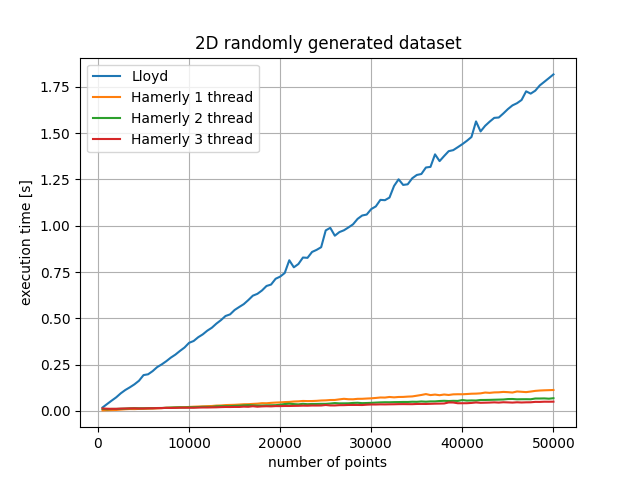
\includegraphics[width = 1\textwidth]{imgs/lh123_2Drnd.png}
    \captionof{figure}{result of the test on the 2D randomly generated dataset}
    \label{fig:lh123_2Drnd}
  \end{center}

  First of all notice that, for all the algorithm, the plot is a straight line. This is as expected if we consider the time complexity of both Lloyd and Hamerly algorithm eq. \ref{eq:lloydcomp} and \ref{eq:hamcomp}, in both cases it is possible to factor the number of points (N) out to obtain an eqation of the type mN.\\

  Talking about the performance, the hamerly algorithm even with 1 thread shows a remarkable speedup with respect to the Lloyd algorithm. Considering the case with 50000 points, the Lloyd algorithm takes 1.81738 seconds while the hamerly algorithm with 1 thread takes 0.113175 seconds, which is approximately 93\% faster. 
  
  By increasing the number of threads, the plot shows an additional speedup: with 2 threads (0.0686808s) the speedup, with respect to the 1 thread hamerly algorithm (0.113175s), is approximately 40\%. As expected, the time taken with 2 threads is not twice the time with 1 thread because some part of the code still be executed sequentially.

  Lastly, the time taken with 3 threads is 0.0500831 which result in an addition 27\% speedup. We can clearly see that by increasing
\end{minipage}
\hspace{0.1in}
\begin{minipage}[b]{0.48\textwidth}
  the number of threads the speedup tends to get smaller, this is as expected and can be proven mathematically. Assuming an ideal speedup, i.e. the time taken by T threads is $\frac{t_1}{T}$ where $t_1$ is the time taken by 1 thread, the time difference between 2 consecutive number of threads can be expressed as
  \begin{equation*}
    \Delta t = t_1 ( \frac{1}{T} - \frac{1}{T + 1} )
  \end{equation*}
  If T tends to infinity $\Delta t$ tends to zero.

  \subsubsection*{3D random dataset}
  To test with a different dataset, the second one used is a three dimension randomly generated dataset (always with 50000 points and 3 centoids).

  The used procedure remains the same used also before, i.e. starting  with a low number of points and increase them gradually (500 points per iteration) to plot the time versus number of points graph.

  \begin{center} 
    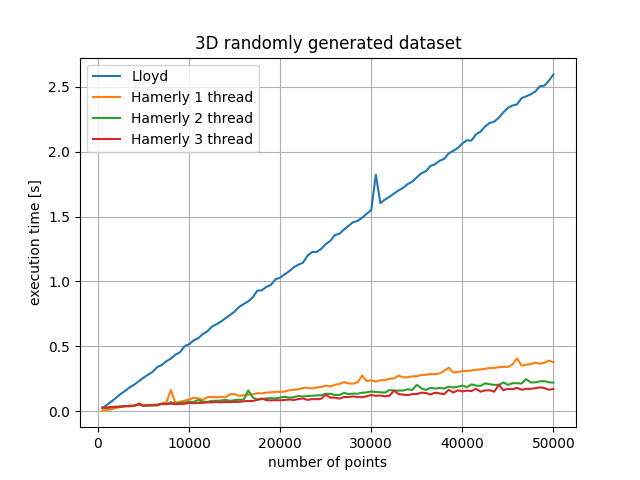
\includegraphics[width = 1\textwidth]{imgs/lh123_3Drnd.png}
    \captionof{figure}{result of the test on the 3D randomly generated dataset}
    \label{fig:lh123_3Drnd}
  \end{center}

  The previous pattern can be seen also in this plot: the lloyd algorithm is considerably slower than the hamerly algorithm with 1 thread and then an additional speedup is obtained by increasing the number of threads.

  By considering the case with 50000 points the time taken by the different algorithms are 2.59356 second for Lloyd, 0.378505 seconds for Hamerly with 1 thread, 0.221699 seconds for Hamerly with 2 threads and 0.173437 seconds.

  The speedup between two consecutive "lines" are respectively: 86\% (lloyd vs hamerly 1 thread), 42\% (hamerly 1 thread vs 2 threads), 22\% (hamerly 2 threads vs 3 threads). Again we notice that as the threads increase the speedup decreases.

  \subsubsection*{Wine quality dataset}
  To test the algorithm with a more realisitc dataset, we downloaded a dataset which contains features about different wines which can be used to group them in classes representing their quality between 0 and 10.

  The number of points in the dataset is 1143, with a dimensionality of 11. The centroids are 10 and were generated by randomly select 10 points between the whole dataset.\\


\end{minipage}

\newpage

\begin{minipage}[b]{0.48\textwidth}
  Other than that, the procedure remains the same but this time the step taken at each iteration to increase the number of points is 9. The result of this test is reported in the followiing graph

  \begin{center} 
    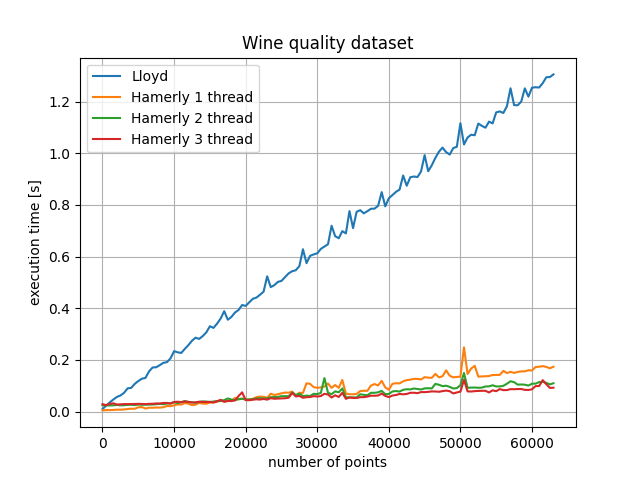
\includegraphics[width = 1\textwidth]{imgs/lh123_wine.png}
    \captionof{figure}{result of the test on wine dataset}
    \label{fig:lh123_wine}
  \end{center}

  By considering the case with 50000 points the time taken by the different algorithms are 1.30501 second for Lloyd, 0.173809 seconds for Hamerly with 1 thread, 0.109867 seconds for Hamerly with 2 threads and 0.0925767 seconds.

  The speedup between two consecutive "lines" are respectively: 87\% (lloyd vs hamerly 1 thread), 34\% (hamerly 1 thread vs 2 threads), 16\% (hamerly 2 threads vs 3 threads).
\end{minipage}
\hspace{0.1in}
\begin{minipage}[b]{0.48\textwidth}
  
\end{minipage}
\end{document}